\documentclass[12pt,a4paper]{article}

\usepackage[utf8]{inputenc}
\usepackage{ctex}
\usepackage{amsmath}
\usepackage{graphicx}
\usepackage{float}
\usepackage{booktabs}
\usepackage{amsfonts}
\usepackage{geometry}
\usepackage{xcolor}
\usepackage{tikz}

\usetikzlibrary{arrows,positioning,shapes,calc,decorations.pathreplacing}

\geometry{margin=1in}

\title{STAEformer 模型架构详解}
\author{}
\date{\today}

\begin{document}

\maketitle

\section{模型整体架构}

\begin{figure}[H]
	\centering
	\begin{tikzpicture}[
			node distance=1cm and 2.5cm,
			box/.style={rectangle, draw, fill=blue!10, minimum width=3cm, minimum height=1cm, font=\small\bfseries, rounded corners},
			arrow/.style={->, thick, >=stealth'},
			sbox/.style={rectangle, draw, fill=#1!20, minimum width=2.2cm, minimum height=0.7cm, font=\tiny}
		]

		\node[box, fill=green!20] (input) at (0,0) {输入 $X$ $(B, T_{in}=12, N, C=3)$};
		\node[box, right=of input] (proj) {Input Projection};
		\node[box, fill=yellow!20, right=of proj] (embed) {时空自适应嵌入融合};
		\node[below=0.5cm of embed, sbox=blue] (inemb) {Input Embed (24维)};
		\node[below=0.5cm of inemb, sbox=green] (todemb) {ToD Embed (24维)};
		\node[below=0.5cm of todemb, sbox=orange] (dowemb) {DoW Embed (24维)};
		\node[below=0.5cm of dowemb, sbox=purple] (adpemb) {Adaptive (80维)};

		\node[box, fill=yellow!30, right=of embed, yshift=1cm] (temporal) {Temporal\\Self-Attention};
		\node[box, fill=orange!30, right=of temporal] (spatial) {Spatial\\Self-Attention};
		\node[box, fill=purple!30, right=of spatial] (ff) {Feed Forward};

		\node[box, fill=red!20, right=of ff] (output) {Mixed Projection};
		\node[box, fill=gray!20, right=of output] (result) {输出 $\hat{Y}$ $(B, T_{out}=12, N, 1)$};

		\draw[arrow] (input) -- (proj);
		\draw[arrow] (proj) -- (embed);
		\draw[arrow] (embed) -- (temporal);
		\draw[arrow] (temporal) -- (spatial);
		\draw[arrow] (spatial) -- (ff);
		\draw[arrow] (ff) -- (output);
		\draw[arrow] (output) -- (result);

		\draw[arrow] (embed.south west) -- (inemb.north);
		\draw[arrow] (inemb.south) -- (todemb.north);
		\draw[arrow] (todemb.south) -- (dowemb.north);
		\draw[arrow] (dowemb.south) -- (adpemb.north);

		\node[draw, dashed, rounded corners, fit=(temporal)(spatial)(ff), label=above:{$\times 3$ STAE Layers}] (layers) {};

	\end{tikzpicture}
	\caption{STAEformer 整体架构图}
\end{figure}

\section{时空自适应嵌入机制}

\begin{figure}[H]
	\centering
	\begin{tikzpicture}[
			node distance=0.5cm and 1cm,
			tensor/.style={rectangle, draw, fill=blue!20, minimum width=1.8cm, minimum height=1.2cm, font=\small},
			embed/.style={rectangle, draw, fill=green!30, minimum width=1.5cm, minimum height=0.8cm},
			arrow/.style={->, thick, >=stealth'},
		]

		\node at (0,0) [tensor] (T) {$T_{in}=12$};
		\node at (3,0) [tensor, right=of T] (N) {$N=207$};
		\node at (6,0) [tensor, right=of N] (D) {$D_{adp}=80$};

		\node[below=1cm of T, text centered, font=\small] {时间步};
		\node[below=1cm of N, text centered, font=\small] {节点数};
		\node[below=1cm of D, text centered, font=\small] {嵌入维度};

		\node[right=3cm of D, tensor, fill=purple!30] (E) {$E_{adp}$};

		\draw[arrow] (T) -- (N);
		\draw[arrow] (N) -- (D);
		\draw[arrow] (D) -- (E) node[midway, above, font=\small] {Expand};

		\node[below=2cm of N, text width=6cm, align=center, font=\small] {%
		自适应嵌入矩阵: $E_{adp} \in \mathbb{R}^{T_{in} \times N \times D_{adp}}$ \\
		参数量: $12 \times 207 \times 80 = 198,720$
		};

	\end{tikzpicture}
	\caption{时空自适应嵌入矩阵结构}
\end{figure}

\section{多头自注意力机制}

\begin{figure}[H]
	\centering
	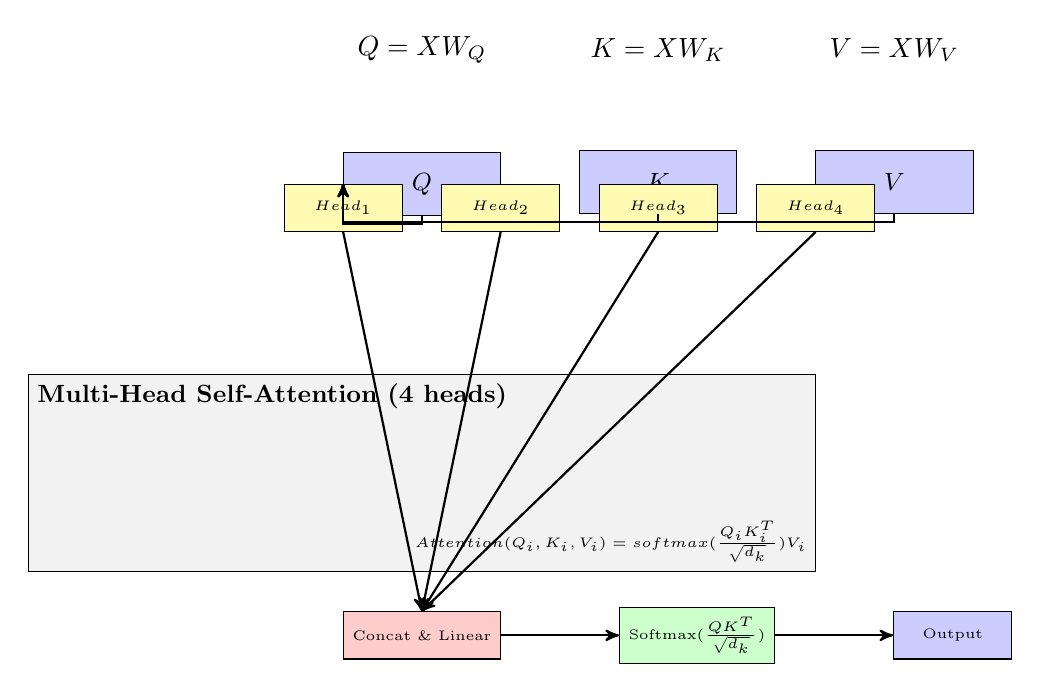
\begin{tikzpicture}[
			node distance=0.5cm and 1.5cm,
			qkv/.style={rectangle, draw, fill=blue!20, minimum width=2cm, minimum height=0.8cm, font=\small},
			head/.style={rectangle, draw, fill=yellow!30, minimum width=1.5cm, minimum height=0.6cm, font=\tiny},
			sbox/.style={rectangle, draw, fill=#1!20, minimum width=1.5cm, minimum height=0.6cm, font=\tiny},
			arrow/.style={->, thick, >=stealth'},
		]

		\node at (0,0) (Q) {$Q = X W_Q$};
		\node at (3,0) (K) {$K = X W_K$};
		\node at (6,0) (V) {$V = X W_V$};

		\node[below=1cm of Q, qkv] (Qbox) {$Q$};
		\node[below=1cm of K, qkv] (Kbox) {$K$};
		\node[below=1cm of V, qkv] (Vbox) {$V$};

		\node[draw, rectangle, fill=gray!10, minimum width=10cm, minimum height=2.5cm, below=2cm of Qbox] (heads) {};

		\foreach \i in {1,...,4} {
				\node[head] (h\i) at ($(\i*2cm-3cm,-2cm)$) {$Head_\i$};
			}

		\node[below=of heads, sbox=red] (concat) {Concat \& Linear};
		\node[right=of concat, sbox=green] (score) {$\text{Softmax}(\frac{QK^T}{\sqrt{d_k}})$};
		\node[right=of score, sbox=blue] (out) {Output};

		\draw[arrow] (Qbox) -- ++(0,-0.5) -| (h1.north);
		\draw[arrow] (Kbox) -- ++(0,-0.5) -| (h1.north);
		\draw[arrow] (Vbox) -- ++(0,-0.5) -| (h1.north);

		\draw[arrow] (h1.south) -- (concat.north);
		\draw[arrow] (h2.south) -- (concat.north);
		\draw[arrow] (h3.south) -- (concat.north);
		\draw[arrow] (h4.south) -- (concat.north);

		\draw[arrow] (concat) -- (score);
		\draw[arrow] (score) -- (out);

		\node at (heads.north west) [anchor=north west, font=\small\bfseries] {Multi-Head Self-Attention (4 heads)};

		\node at (heads.south east) [anchor=south east, font=\tiny] {%
			$Attention(Q_i, K_i, V_i) = softmax(\frac{Q_i K_i^T}{\sqrt{d_k}}) V_i$
		};

	\end{tikzpicture}
	\caption{多头自注意力机制}
\end{figure}

\section{时空交替Transformer层}

\begin{figure}[H]
	\centering
	\begin{tikzpicture}[
			node distance=0.3cm and 1.2cm,
			layer/.style={rectangle, draw, fill=blue!25, minimum width=2.5cm, minimum height=0.9cm, font=\small\bfseries, rounded corners},
			arrow/.style={->, thick, >=stealth'},
		]

		\node[layer] (input) at (0,0) {Input $X$};
		\node[layer, fill=green!25, right=of input] (ln1) {LayerNorm};
		\node[layer, fill=yellow!30, right=of ln1] (attnt) {Temporal Attn};
		\node[layer, fill=green!25, right=of attnt] (ln2) {LayerNorm};
		\node[layer, fill=orange!30, right=of ln2] (attns) {Spatial Attn};
		\node[layer, fill=green!25, right=of attns] (ln3) {LayerNorm};
		\node[layer, fill=purple!25, right=of ln3] (ff) {Feed Forward};
		\node[layer, fill=green!25, right=of ff] (ln4) {LayerNorm};
		\node[layer, right=of ln4] (output) {Output};

		\draw[arrow] (input) -- (ln1);
		\draw[arrow] (ln1) -- (attnt);
		\draw[arrow] (attnt) -- (ln2);
		\draw[arrow] (ln2) -- (attns);
		\draw[arrow] (attns) -- (ln3);
		\draw[arrow] (ln3) -- (ff);
		\draw[arrow] (ff) -- (ln4);
		\draw[arrow] (ln4) -- (output);

		\draw[dashed, thick, rounded corners] (-1.5cm, -1.2cm) rectangle (11cm, 1.5cm)
		node[midway, below, yshift=-0.3cm, font=\small] {STAE Layer ($\times 3$)};

	\end{tikzpicture}
	\caption{时空交替注意力层结构}
\end{figure}

\section{数据流与维度变化}

\begin{figure}[H]
	\centering
	\begin{tikzpicture}[
			node distance=0.5cm and 2cm,
			box/.style={rectangle, draw, fill=#1!20, minimum width=4cm, minimum height=1cm, font=\small, align=center},
			arrow/.style={->, thick, >=stealth'},
		]

		\node[box=blue] (x0) at (0,0) {$X$ $(B, 12, 207, 3)$\\\footnotesize 原始输入};
		\node[box=blue, right=of x0] (x1) {$X_{proj}$ $(B, 12, 207, 24)$\\\footnotesize Input Projection};
		\node[box=green, right=of x1] (x2) {$X_{fused}$ $(B, 12, 207, 152)$\\\footnotesize 嵌入融合};

		\node[box=yellow, below=2cm of x2, xshift=2cm] (x3) {$X_{temporal}$\\\footnotesize Temporal Attn};
		\node[box=orange, right=of x3] (x4) {$X_{spatial}$\\\footnotesize Spatial Attn};
		\node[box=purple, right=of x4] (x5) {$X_{ff}$\\\footnotesize Feed Forward};

		\node[box=red, below=2cm of x5, xshift=-2cm] (x6) {$X_{mixed}$\\\footnotesize Mixed Proj};
		\node[box=gray, left=of x6] (x7) {$\hat{Y}$ $(B, 12, 207, 1)$\\\footnotesize 预测输出};

		\draw[arrow] (x0) -- (x1);
		\draw[arrow] (x1) -- (x2);
		\draw[arrow] (x2) -- ++(0,-1) -| (x3.north);
		\draw[arrow] (x3) -- (x4);
		\draw[arrow] (x4) -- (x5);
		\draw[arrow] (x5) -- ++(0,-1) -| (x6.north);
		\draw[arrow] (x6) -- (x7);

	\end{tikzpicture}
	\caption{数据流与维度变化}
\end{figure}

\section{Mixed Projection 输出映射}

\begin{figure}[H]
	\centering
	\begin{tikzpicture}[
			node distance=0.5cm and 1.8cm,
			box/.style={rectangle, draw, fill=#1!20, minimum width=3.5cm, minimum height=0.9cm, font=\small\bfseries},
			arrow/.style={->, thick, >=stealth'},
		]

		\node[box=blue] (input) at (0,0) {$X$ $(B,T_{in},N,D)$};
		\node[right=of input, box=gray] (T) {Transpose};
		\node[right=of T, box=gray] (R) {Reshape};
		\node[right=of R, box=purple] (L) {Linear};
		\node[right=of L, box=gray] (V) {View};
		\node[right=of V, box=gray] (T2) {Transpose};
		\node[right=of T2, box=red] (out) {$\hat{Y}$};

		\node[below=0.5cm of T, font=\tiny] {$(B,N,T_{in},D)$};
		\node[below=0.5cm of R, font=\tiny] {$(B,N,T_{in} \cdot D)$};
		\node[below=0.5cm of L, font=\tiny] {$(B,N,T_{out})$};
		\node[below=0.5cm of V, font=\tiny] {$(B,N,T_{out},1)$};
		\node[below=0.5cm of T2, font=\tiny] {$(B,T_{out},N,1)$};

		\draw[arrow] (input) -- (T);
		\draw[arrow] (T) -- (R);
		\draw[arrow] (R) -- (L);
		\draw[arrow] (L) -- (V);
		\draw[arrow] (V) -- (T2);
		\draw[arrow] (T2) -- (out);

	\end{tikzpicture}
	\caption{Mixed Projection 输出映射}
\end{figure}

\section{模型参数配置}

\begin{table}[H]
	\centering
	\caption{STAEformer 默认配置参数}
	\begin{tabular}{lr}
		\toprule
		参数名称                               & 默认值 \\
		\midrule
		节点数 (num\_nodes)                   & 207 \\
		输入时间步 (in\_steps)                  & 12  \\
		输出时间步 (out\_steps)                 & 12  \\
		每日步数 (steps\_per\_day)             & 288 \\
		输入维度 (input\_dim)                  & 3   \\
		输出维度 (output\_dim)                 & 1   \\
		输入嵌入维度 (input\_embedding\_dim)     & 24  \\
		时间嵌入维度 (tod\_embedding\_dim)       & 24  \\
		星期嵌入维度 (dow\_embedding\_dim)       & 24  \\
		自适应嵌入维度 (adaptive\_embedding\_dim) & 80  \\
		前馈网络维度 (feed\_forward\_dim)        & 256 \\
		注意力头数 (num\_heads)                 & 4   \\
		Transformer层数 (num\_layers)        & 3   \\
		模型总维度 (model\_dim)                 & 152 \\
		\bottomrule
	\end{tabular}
\end{table}

\end{document}